\chapter{Markov Decision Processes}

\section{Introduction}
Reinforcement learning consists in teaching an agent how to behave using 
observations from its environment with the goal of maximizing 
future rewards that it receives in response to its behavior. 
The set-up consists of an \emph{agent}, 
which is the learner or decision maker and the \emph{enviroment}, which is 
the thing that the agent interacts with, comprising everything outside the agent. 
The agent and the environment interact in discrete time steps. At a given time 
step~$t$, the agent takes an \emph{action} and the environment responds by 
presenting a new state and a scalar feedback signal called the \emph{reward}.

\begin{figure}[h]
\begin{center}
    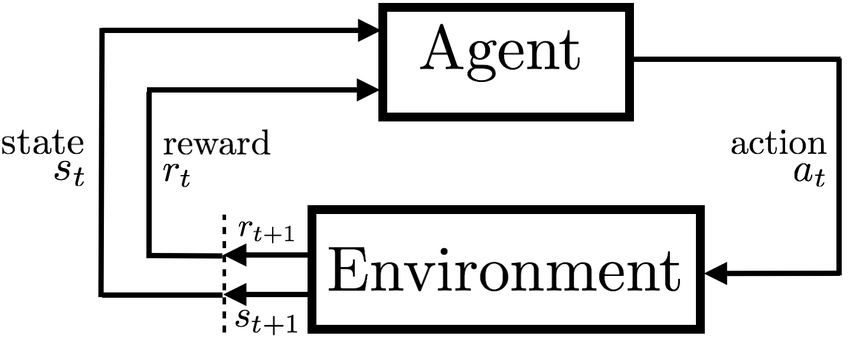
\includegraphics[scale=0.3]{RLAgentEnvironment.png}
\end{center}   
\caption{The agent and the environment}
\end{figure}


Problems in reinforcement learning are typically formulated in the formal
setting of a Markov Decision Process (MDP). An MDP is a five-tuple
$\angular{\states, \actions, p, \rewards, \discount}$
\begin{itemize}
    \item a set $\states$ of states
    \item a set $\actions$ of actions
    \item a set $\rewards$ of rewards
    \item a probability function
        $p \colon \states \times \rewards \times \states \times \actions \rightarrow [0, 1]$
    \item a discount factor $\discount \in [0, 1]$
\end{itemize}

The probablity function~$p$ defines the dynamics of the MDP. It tells us what 
the most likely next state and reward combination are given the current state 
and the action taken by the agent. 
\begin{equation}
    p(s', r \mid s, a) \defn \Prone{S_{t + 1} = s', R_{t + 1} = r \mid S_t = s, A_t = a}.
\end{equation} 
In the above equation, we assume that the probability does \emph{not} depend 
on the time step~$t$. Such an MDP is called \emph{stationary}. 
Since this is a probablity distribution, for all $s \in \states$ and for all 
$a \in \actions$,
\begin{equation}
    \sum_{s' \in \states} \sum_{r \in \rewards} p(s', r \mid s, a) = 1.
\end{equation}
We also define a state-transition probability function 
$p \colon \states \times \actions \times \states \rightarrow [0, 1]$ defined as:
\begin{equation}
    p(s' \mid s, a) \defn \sum_{r \in \rewards}  p(s', r \mid s, a).
\end{equation}

In response to the action taken by the agent, the environment provides it a 
scalar rewards at each time step. The total reward of the agent in time step $t$ is
defined as
\begin{equation}
    G_t \defn \sum_{k = 0}^{\infty} R_{t + k + 1}.
\end{equation}
With infinite time horizons, this reward could go to infinity. To prevent this,
one uses a discounting factor $\gamma \in [0, 1]$ and defines the total reward as
\begin{equation}
    G_t \defn R_{t + 1} + \gamma \cdot R_{t + 2} + \gamma^2 \cdot R_{t + 3} + \cdots 
\end{equation}

\subsection{Policy and Value Functions}
A \emph{policy}~$\policy$ is a mapping from states to probabilities of selecting each possible 
action. 
\begin{equation}
    \policy (a \mid s) \defn \Prone {A_t = a \mid S_t = s}.
\end{equation}
Note that this probability distribution does not depend on the time step~$t$.

\begin{exer}
If the current state is $S_t$, and actions are selected according to a stochastic
policy $\policy$, then what is the expectation of $R_{t + 1}$ in terms of 
$\policy$ and the four-argument function $p$?
\end{exer}
\begin{solution}
Let us assume that the current state $S_t = s$. We may write 
$\Exptwo{\policy}{R_{t + 1} \mid S_t = s}$ as:
\begin{align*}
    \Exptwo{\policy}{R_{t + 1} \mid S_t = s} 
        & = \sum_{r \in \rewards} r \cdot \Prtwo{\policy}{R_{t + 1} = r \mid S_t = s} \\
        & = \sum_{r \in \rewards} r \cdot \sum_{a \in \actions} 
                \Prtwo{\policy}{R_{t + 1} = r\mid S_t = s, A_t = a} 
                    \cdot \Prtwo{\policy}{A_{t} = a \mid S_t = s} \\ 
        & = \sum_{r \in \rewards} r \cdot \sum_{a \in \actions} 
            \sum_{s' \in \states} p(s', r \mid s, r) \cdot \policy (a \mid s) 
\end{align*}
\qed
\end{solution}

The \emph{value function} of a state~$s$ under a policy~$\policy$, denoted 
$v_{\policy}(s)$, is the expected return when starting in state~$s$ and 
following $\policy$ thereafter. For an MDP, we may write the value function as:
\begin{equation}
    v_{\policy}(s) \defn \Exptwo{\policy}{G_t \mid S_t = s} 
        = \Exptwo{\policy}{\sum_{k = 0}^{\infty} \discount^{k} \cdot R_{t + k + 1} \bigm\vert S_t = s }.
\end{equation}
The function $v_{\policy}(s)$ is called the \emph{state-value function} of the policy $\policy$.

We also define the value of taking an action $a$ in state $s$ under a policy $\policy$, 
denoted $q_{\policy}(s, a)$, as the expected return when starting in state $s$, 
taking action $a$ and following $\policy$ thereafter.
\begin{equation}
    q_{\policy}(s, a) \defn \Exptwo{\policy}{G_t \mid S_t = s, A_t = a} 
        = \Exptwo{\policy}{\sum_{k = 0}^{\infty} \discount^{k} \cdot R_{t + k + 1} \bigm\vert S_t = s, A_t = a}.
\end{equation}
The function $q_{\policy}(s, a)$ is the \emph{action-value function} of the policy $\policy$. 

\begin{exer}
Give an equation for $v_{\policy}$ in terms of $q_{\policy}$ and $\policy$.
\end{exer}
\begin{solution}
We may write $v_{\policy}(s)$ as:
\begin{align*}
    v_{\policy}(s) & \defn \Exptwo{\policy}{G_t \vert S_t = s} \\
                   & = \sum_{a \in \actions} \Exptwo{\policy}{G_t \vert S_t = s, A_t = a} 
                        \cdot \Prtwo{\policy}{A_t = a \vert S_t = a} \\
                   & = \sum_{a \in \actions} q_{\policy}(s, a) \policy (a \vert s).
\end{align*}
\qed
\end{solution}

\begin{exer}
Give an equation for $q_{\policy} (s, a)$ in terms of $v_{\policy}$ and the 
four parameter function $p$. 
\end{exer}
\begin{solution}
\begin{align*}
    q_{\pi}(s, a) & \defn \Exptwo{\policy}{R_{t + 1} + \discount \cdot R_{t + 2} + \discount^2 \cdot R_{t + 3} + \cdots \vert S_t = s, A_t = a} \\
                  & = \Exptwo{\policy}{R_{t + 1} \vert S_t = s, A_t = a} + 
                    \discount \cdot \Exptwo{\policy}{G_{t + 1} \vert S_t = s, A_t = a} \\
                  & = \sum_{r \in \rewards} r \cdot \Prtwo{\policy}{R_{t + 1} = r \vert S_t = s, A_t = a} + \\
                  & \quad \quad \discount \cdot \sum_{s' \in \states} \Exptwo{\policy}{G_{t + 1} \vert S_{t + 1} = s', S_t = s, A_t = a}
                        \cdot \Prtwo{\policy}{S_{t + 1} = s' \vert S_t = s, A_t = a} \\ 
                  & = \sum_{r \in \rewards} r \cdot \sum_{s' \in \states} p(s', r \vert s, a) + 
                    \discount \cdot \sum_{s' \in \states} \Exptwo{\policy}{G_{t + 1} \vert S_{t + 1} = s'} 
                        \cdot \sum_{r \in \rewards} p(s', r \vert s, a) \\
                  & = \sum_{r \in \rewards} \sum_{s' \in \states} \left ( r + \discount \cdot v_{\policy}(s') \right )p(s', r \vert s, a).
\end{align*}
\end{solution}
